\section{Ecosistemas}

Todos los seres vivos se distribuyen en los medios formando parte de ecosistemas. (Figura \ref{fig:tipos-ecosistemas})

\begin{figure}[!ht]
    \centering
    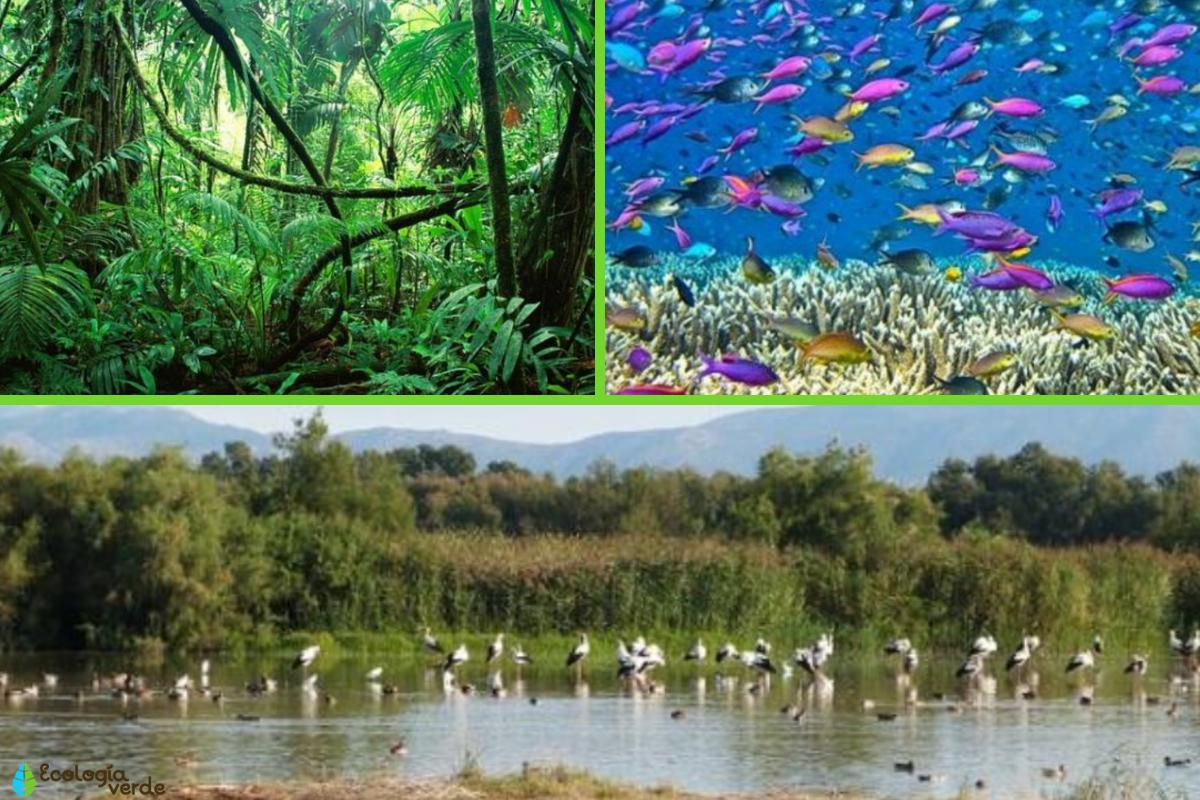
\includegraphics[width=0.7\linewidth]{Tema1/20_Tipos_ecosistemas.jpg}
    \caption{Tipos de ecosistemas}
    \label{fig:tipos-ecosistemas}
\end{figure}

\subsection{Elementos de los ecosistemas}

Un \textbf{ecosistema} es un conjunto formado por un lugar y sus condiciones físicas (llamado \textbf{biotopo}), por una comunidad de seres vivos de varios tipos (llamada \textbf{biocenosis}) y por las relaciones que se dan entre todos estos elementos.

\begin{itemize}
    \item El \textbf{biotopo}. El \textbf{biotopo} de un ecosistema es el conjunto formado por los componentes no vivos de un lugar, como las rocas y el suelo, el aire y el clima, el agua, la luz... Estos componentes varían mucho de unos lugares a otros y determinan que existan varios tipos de ecosistemas, con comunidades de seres vivos propias de esas condiciones.
    \item La \textbf{biocenosis}. La \textbf{biocenosis} o comunidad es el conjunto completo de seres vivos que forman parte de un ecosistema. A su vez, la comunidad de seres vivos de un ecosistema está formada por varias poblaciones. Una \textbf{población} es un conjunto de seres vivos de una misma especie que vive en un ecosistema.
\end{itemize}

\subsection{Relaciones y equilibrio}

En todo ecosistema se dan relaciones entre sus elementos (Figura \ref{fig:relaciones-alimentarias-ecosistema}). Por ejemplo, entre todos los seres vivos y el agua, entre el suelo y las plantas, entre unos seres vivos y otros... Si las relaciones en un ecosistema se mantienen estables y permiten la supervivencia de los seres vivos que lo componen, se dice que ese ecosistema está en \textbf{equilibrio}. De entre todas las relaciones que se dan en un ecosistema, se pueden destacar las \textbf{relaciones alimentarias} o \textbf{tróficas}, que se dan cuando los seres vivos intentan obtener los nutrientes que necesitan. Según esto, los seres vivos de un ecosistema pueden ser:
\begin{itemize}
    \item \textbf{Productores}. Son los seres vivos con \textbf{nutrición autótrofa}, como las \textbf{plantas}, las \textbf{algas} o algunas \textbf{bacterias}. Estos seres son capaces de fabricar (producir) sus nutrientes a partir de agua, dióxido de carbono y minerales que toman del biotopo.
    \item \textbf{Consumidores}. Son los seres vivos con \textbf{nutrición heterótrofa}, como los \textbf{animales} y algunos \textbf{protozoos}, que deben alimentarse de otros seres vivos o de sus partes para obtener nutrientes.
    \item \textbf{Descomponedores}. Son \textbf{bacterias} y \textbf{hongos} capaces de obtener nutrientes y energía \textbf{descomponiendo los restos de seres vivos} en sustancias como agua, gases y minerales, que devuelven al medio para que las utilicen los demás seres vivos.
\end{itemize}

\begin{figure}[!ht]
    \centering
    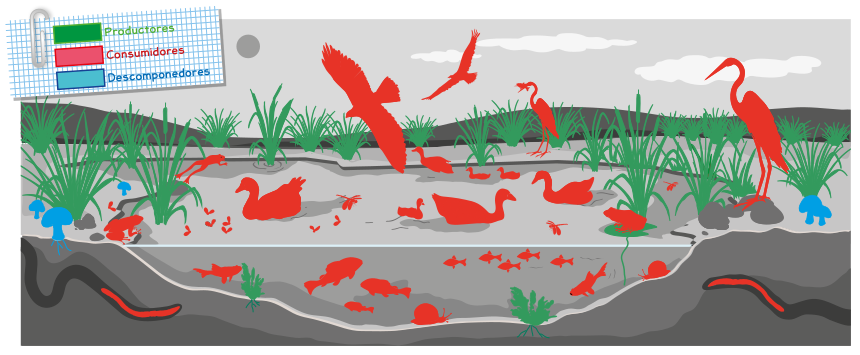
\includegraphics[width=0.8\linewidth]{Tema1/21_Relaciones_alimentarias.png}
    \caption{Relaciones alimentarias en el ecosistema}
    \label{fig:relaciones-alimentarias-ecosistema}
\end{figure}

\subsection{Cadenas y redes tróficas}

Las relaciones tróficas de un ecosistema pueden representarse con unos esquemas llamados \textbf{cadenas y redes tróficas} (Figura: \ref{fig:cadenas-redes-troficas}) en los que se indica, mediante flechas, cómo circula el alimento entre un grupo de seres del ecosistema. Las flechas de estos gráficos siempre apuntan hacia el ser vivo que obtiene el alimento.
\begin{itemize}
    \item \textbf{Las cadenas tróficas.} En una cadena trófica se representa una \textbf{relación lineal de seres vivos} que obtienen su alimento unos de los otros. En ella se parte de un productor, del que se alimenta un consumidor, del que se alimenta otro consumidor...
    \item \textbf{Las redes tróficas.} En las redes tróficas se representan \textbf{varias cadenas tróficas relacionadas}. Se ajustan más a las relaciones tróficas reales del ecosistema, porque reflejan el hecho de que cada tipo de ser vivo puede tener varias fuentes de alimento, o puede servir como alimento a algunos tipos de seres.
\end{itemize}

\begin{figure}[!ht]
    \centering
    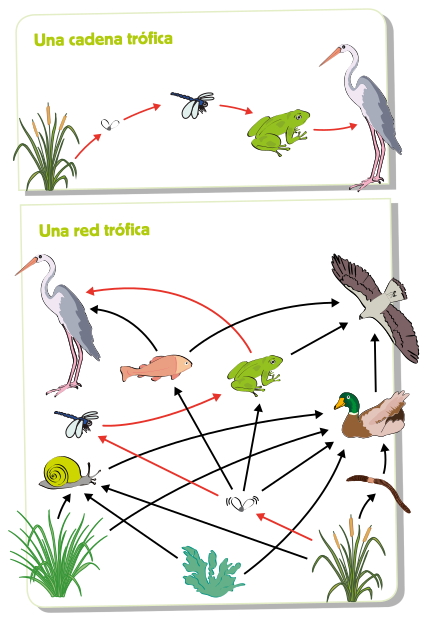
\includegraphics[width=0.4\linewidth]{Tema1/22_Cadenas_Redes_Troficas.png}
    \caption{Cadenas y redes tróficas}
    \label{fig:cadenas-redes-troficas}
\end{figure}

\subsection{Las adaptaciones}

Las especies que forman la biocenosis o comunidad están \textbf{adaptadas} para sobrevivir y reproducirse en el ecosistema del que forman parte. Las \textbf{adaptaciones} son características de estos seres vivos que les permiten:
\begin{itemize}
    \item \textbf{Aprovechar o soportar las condiciones del biotopo}: obtener oxígeno, conseguir agua, desplazarse, resistir el clima...
    \item \textbf{Relacionarse con otros seres vivos}: alimentarse, defenderse, asociarse, aparearse...
\end{itemize}
Las adaptaciones pueden ser partes u órganos del cuerpo de los seres vivos; por ejemplo, las aletas o las branquias de los animales acuáticos o el tallo que almacena agua en los cactus. También pueden ser características del funcionamiento o del comportamiento de los seres vivos, como la pérdida de la hoja de los robles en otoño, los cantos de cortejo de las aves...

\subsection{El ser humano y los ecosistemas}

Como los demás seres vivos, las personas formamos parte de ecosistemas. Nuestra principal adaptación, nuestra inteligencia, nos hace capaces de integrarnos y prosperar en casi todos los ecosistemas del planeta. Somos consumidores muy eficaces, ya que obtenemos alimentos de otros seres vivos que cazamos, recolectamos, criamos o cultivamos. Pero además, de los ecosistemas obtenemos materiales, agua, aire, energía, espacio...

\vspace{3mm}
Por estas razones, nos hemos extendido por casi todo el planeta y hemos tenido gran éxito. Pero nuestra presencia está produciendo daños y desequilibrios en muchos ecosistemas. Los principales son los siguientes:
\begin{itemize}
    \item \textbf{El agotamiento de los recursos}. Consumimos tantos recursos y tan rápido que no da tiempo a que se regeneren de forma natural. Así, por ejemplo:
    \begin{itemize}
        \item Estamos agotando recursos como el petróleo, los minerales o el agua dulce.
        \item Estamos poniendo en \textbf{peligro de extinción} a muchos seres vivos que recolectamos o capturamos en exceso y no tienen tiempo de recuperarse mediante la reproducción.
    \end{itemize}
    \item \textbf{La alteración o destrucción de ecosistemas}. Nuestras actividades hacen que los ecosistemas se alteren o incluso se destruyan, con la consiguiente extinción de muchos de los seres que contienen. Las principales causas son:
    \begin{itemize}
        \item La \textbf{contaminación} del aire, del agua o del suelo con sustancias perjudiciales.
        \item La \textbf{acumulación de residuos} tanto en medios terrestres como acuáticos.
        \item La \textbf{ocupación del territorio} con cultivos, pastos, poblaciones, instalaciones...
        \item La \textbf{introducción de especies} en ecosistemas que no son los suyos. Estas especies provocan graves desequilibrios en esos ecosistemas.
    \end{itemize}
\end{itemize}